
\PassOptionsToPackage{colorlinks,linkcolor={blue},citecolor={blue},urlcolor={blue},breaklinks=true,final}{hyperref}
\PassOptionsToPackage{dvipsnames}{xcolor}
\documentclass[xcolor={dvipsnames,svgnames},aspectratio=169]{beamer}

\usepackage{fontawesome5}
\usepackage{booktabs} % For better table formatting
\usepackage{listings}
\usepackage{tabularx}


\lstset{
  tabsize = 4, %% set tab space width
  showstringspaces = false, %% prevent space marking in strings, string is defined as the text that is generally printed directly to the console
  numbers = left, %% display line numbers on the left
  commentstyle = \color{purple!60}, %% set comment color
  keywordstyle = \color{blue}, %% set keyword color
  stringstyle = \color{red}, %% set string color
  rulecolor = \color{black}, %% set frame color to avoid being affected by text color
  basicstyle = \small \ttfamily , %% set listing font and size
  breaklines = true, %% enable line breaking
  numberstyle = \tiny,
}

\title{Concurrent Programming}
\subtitle{Week 18 (Lecture 7) : \textbf{Liveness hazards and performance}}
\author{Stelios Tsampas}
\institute{
  \faEnvelope \; stelios@imada.sdu.dk
  \qquad
  \faGlobe \;
  \href{https://www.steliostsampas.com}{https://www.steliostsampas.com}
  \\\\\
  \faGithub \; stelios-tau/cp-2025
  \qquad\;\;
    \faDiscord \; cp-2025
}
\date{\today}

\titlegraphic{\includegraphics[height=0.6cm,keepaspectratio]{../media/sdu-black.eps}}

\usetheme[block=fill]{metropolis}


%\usepackage{pres-common}
\usepackage{textpos}
\usepackage{centernot}

% \newcommand{\Goesv}[3]{\ensuremath{#1 \xRightarrow{~#3~} #2}}
% \newcommand{\goesv}[3]{\ensuremath{#1 \xrightarrow{~#3~} #2}}

% \usepackage{etex}
% \usepackage{semantic}

\usepackage[utf8]{inputenc}
\usepackage[english]{babel}
\usepackage{tikz}
\usepackage{hyperref}

\usetikzlibrary{arrows,shapes,matrix}
\usetikzlibrary{backgrounds}
\usetikzlibrary{arrows.meta}
\usetikzlibrary{positioning}
\usetikzlibrary{automata}
\usetikzlibrary{mindmap}
\usetikzlibrary{shapes.callouts}
\usetikzlibrary{decorations.text}
\usetikzlibrary{tikzmark}
\usetikzlibrary{calc}
\usetikzlibrary{overlay-beamer-styles}
\usetikzlibrary{shapes.geometric}
\usepackage{pgfplots}


\tikzset{onslide/.code args={<#1>#2}{%
    \only<#1>{\pgfkeysalso{#2}} % \pgfkeysalso doesn't change the path
  }}

\setbeamercolor{mygray}{bg=Gray!20}

\tikzset{temporal/.code args={<#1>#2#3#4}{%
    \temporal<#1>{\pgfkeysalso{#2}}{\pgfkeysalso{#3}}{\pgfkeysalso{#4}} % \pgfkeysalso doesn't change the path
  }}

\tikzstyle{highlight}=[fill=green!50]
\tikzstyle{hgreen}=[fill=green!20]
\tikzstyle{hred}=[fill=red!50]
\tikzstyle{hblue}=[fill=blue!50]
\tikzstyle{hgray}=[fill=gray!50]

\addtobeamertemplate{frametitle}{}{%
\begin{textblock*}{100mm}(\textwidth-2cm,-0.86cm)
\includegraphics[height=0.6cm,keepaspectratio]{../media/sdu-white.eps}
\end{textblock*}}


%\usepackage{tikz-cd}
% \usepackage{wasysym}
% \usepackage{color}
% \usepackage[matrix,arrow]{xy}
% \xyoption{all}
% \SelectTips{cm}{}
% % \usepackage{cite}
% \usepackage{amsthm}
% \usepackage{amsmath}
% \usepackage{bbold}
% % \usepackage[bbgreekl]{mathbbol}
% \usepackage{amssymb}
% \usepackage{pifont}
% \usepackage{mathtools}
% \usepackage{amsbsy}
% % \usepackage{paralist}
% \usepackage{shadethm}
% % \usepackage{fancyhdr}
% \usepackage{stmaryrd}
% \usepackage{wasysym}
% \usepackage{graphicx}
% \usepackage{tabularx}
% \usepackage{dsfont}
% \usepackage{ulem}




%\bibliography{mainBiblio}

%\includeonlyframes{current}
\begin{document}

\frame{\titlepage}

\def\firstcircle{(0,0) circle (2cm)}
\def\secondcircle{(1.4,1.4) circle (2cm)}
\def\thirdcircle{(0:2.4) circle (2cm)}

\begin{frame}{Outline}
  \tableofcontents
\end{frame}

\section{Recap}

\begin{frame}[fragile]
  \frametitle{Previously on CP}

  Last lecture, we looked at...

  \begin{itemize}
  \item[\faBook]<1-> The fundamental producer-consumer pattern, in which the
    creation of tasks is separated from their undertaking.
    \begin{itemize}
    \item[\faBook]<1-> \emph{Producer} threads create tasks, \emph{consumers}
      complete them.
    \end{itemize}
  \item[\faBook]<1-> Low-level thread coordination primitives,
    \begin{itemize}
    \item[\faBook]<1-> namely \texttt{wait()}, \texttt{notify()} and
      \texttt{notifyAll()}.
    \end{itemize}
  \item[\faBook]<1-> The \texttt{BlockingQueue} interface as an efficient way to
    manage tasks.
  \item[\faBook]<1-> The \texttt{Executor} as an efficient, more advanced way to
    manage tasks.
  \end{itemize}

  \vspace{0.4cm}

  \begin{block}<2->{\faLightbulb \quad Key takeaway}
    The producer-consumer pattern is a ubiquitous pattern arises naturally in
    many concurrency scenarios (it is not the only one). The developer has many
    tools to manage tasks in an efficient and reliable manner.
  \end{block}

\end{frame}

\begin{frame}[fragile]
  \frametitle{This week's topics}

  This week, we will look at...

  \begin{itemize}
  \item[\faBook]<1-> Liveness issues!
  \item[\faBook]<1-> Performance and scalability considerations!
  \item[\faBook]<1-> Streams in parallel!
  \item[\faBook]<1-> Some information on the exam!
  \end{itemize}
\end{frame}

\begin{frame}[fragile]
  \frametitle{Pitfalls in concurrency}

  In concurrent programming, there are three main classes of pitfalls:

  \begin{itemize}
  \item[\faUserInjured]<1-> (Thread) safety issues (e.g. race conditions,
    publishing etc.).
  \item[\faUserInjured]<2-> \textbf{Liveness issues}.
  \item[\faUserInjured]<3-> \textbf{Performance}.
  \end{itemize}

\end{frame}

\section{Liveness Hazards}



\begin{frame}[fragile]
  \frametitle{Liveness in Concurrency}

  \begin{block}<1->{\faSearch \quad Liveness}
    Something good eventually happens.
  \end{block}

  In concurrent programs, \textbf{liveness hazards} occur when:

  \begin{itemize}
  \item[\faUserInjured]<1-> Threads \textbf{don't make progress} toward their
    goals.
  \item[\faUserInjured]<1-> Systems appear stuck or unresponsive.
  \end{itemize}
\end{frame}

\begin{frame}[fragile]
  \frametitle{Liveness in Concurrency}

  \begin{block}<1->{\faSearch \quad Liveness}
    \emph{Something good eventually happens.}
  \end{block}

  In concurrent programs, \textbf{liveness hazards} occur when:

  \begin{itemize}
  \item[\faUserInjured]<1-> Threads \textbf{don't make progress} toward their
    goals.
  \item[\faUserInjured]<1-> Systems appear stuck or unresponsive.
  \end{itemize}

  The three classic problems are \textbf{Deadlock}, \textbf{starvation} and
  \textbf{livelock}.

  \vspace{0.2cm}

  \begin{block}<2->{\faExclamationTriangle \quad Warning}
    Liveness issues are elusive, do not manifest easily, so extra care is
    needed.
  \end{block}

\end{frame}

\begin{frame}[fragile]
  \frametitle{\faSkull \quad Deadlock}

  \begin{block}<1->{\faSearch \quad What is a deadlock?}
    The condition during execution where two or more threads are blocked
    forever, waiting for each other.
  \end{block}

    \vspace{0.5cm}

    \begin{block}<2->{\faSearch \quad When does it occur?}
    Multiple patterns, typically involves a \textbf{cyclic dependency} of locks
    between multiple threads.
  \end{block}

  \vspace{0.5cm}

  \begin{block}<3->{\faSearch \quad Real-world example}
    Two cars are stuck on a one-way bridge, blocking each other.
  \end{block}
\end{frame}

\begin{frame}[fragile]
  \frametitle{\faSkull \quad Deadlock example (1)}

\begin{lstlisting}[basicstyle=\fontsize{8}{9}\selectfont\ttfamily, language = Java ,
frame = trBL , firstnumber = last , escapeinside={(*@}{@*)},numbers=none]
Thread t1 = new Thread(() -> {
    synchronized (lockA) {
        synchronized (lockB) { System.out.println("Thread 1 done"); }
    }
});

Thread t2 = new Thread(() -> {
    synchronized (lockB) {
        synchronized (lockA) { System.out.println("Thread 2 done"); }
    }
});
\end{lstlisting}

    \uncover<2->{
    \begin{tikzpicture}[overlay, remember picture]
      \node[xshift=10.4cm,yshift=3cm,starburst,starburst points=40,
      align=center,fill=yellow, opacity=1,draw=red, line width=2pt]
      {\textbf{\texttt{t1} waits B, \texttt{t2} waits A \faSkullCrossbones!}};
    \end{tikzpicture}}

  \begin{block}<3->{\faLightbulb \quad Key takeaway}
    Threads accessing \textbf{multiple} locks in \textbf{different} order is a source of deadlocks.
  \end{block}
\end{frame}

\begin{frame}[fragile]
  \title{Wait-for-graph}

  \begin{center}
    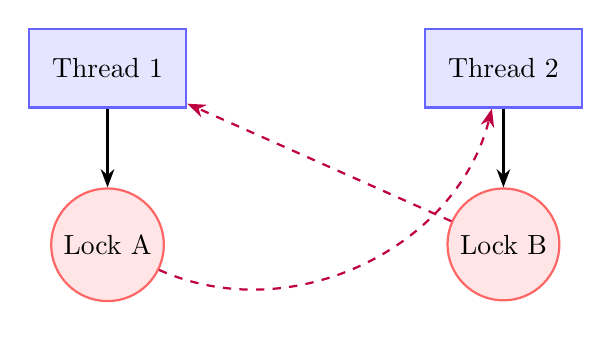
\begin{tikzpicture}[
      thread/.style={rectangle, draw=blue!60, fill=blue!10, thick, minimum width=2cm, minimum height=1cm},
      lock/.style={circle, draw=red!60, fill=red!10, thick, minimum size=1cm},
      arrow/.style={->, thick, >=Stealth}
      ]

      % Nodes
      \node[thread] (T1) {Thread 1};
      \node[lock, below=of T1] (A) {Lock A};

      \node[thread, right=3cm of T1] (T2) {Thread 2};
      \node[lock, below=of T2] (B) {Lock B};

      % Arrows
      \draw[arrow] (T1) -- (A);
      \draw[arrow] (T2) -- (B);
      \draw[arrow,purple,dashed] (B) -- (T1);
      \draw[arrow,purple,dashed] (A) to[bend right=50] (T2);

    \end{tikzpicture}
  \end{center}

  \begin{block}<2->{\faPuzzlePiece \quad What is wrong?}
    \uncover<3>{There's a cyclic dependency, meaning we have a deadlock!}
  \end{block}

\end{frame}

\begin{frame}[fragile]
  \frametitle{\faSkull \quad Deadlock example (2)}

\begin{lstlisting}[basicstyle=\fontsize{8}{9}\selectfont\ttfamily, language = Java ,
frame = trBL , firstnumber = last , escapeinside={(*@}{@*)},numbers=none]
Thread t1 = new Thread(() -> {
    synchronized (lockA) {
        synchronized (lockB) { System.out.println("Thread 1 done"); }
    }
});
Thread t2 = new Thread(() -> {
    synchronized (lockB) {
        synchronized (lockC) { System.out.println("Thread 2 done"); }
    }
});
Thread t3 = new Thread(() -> {
    synchronized (lockC) {
        synchronized (lockA) { System.out.println("Thread 3 done"); }
    }
});
\end{lstlisting}

  \begin{block}<2->{\faLightbulb \quad Key takeaway}
    Cyclic dependency of resources can occur with any number of threads.
  \end{block}
\end{frame}

\begin{frame}[fragile]
  \title{Wait-for-graph}

  \begin{center}
    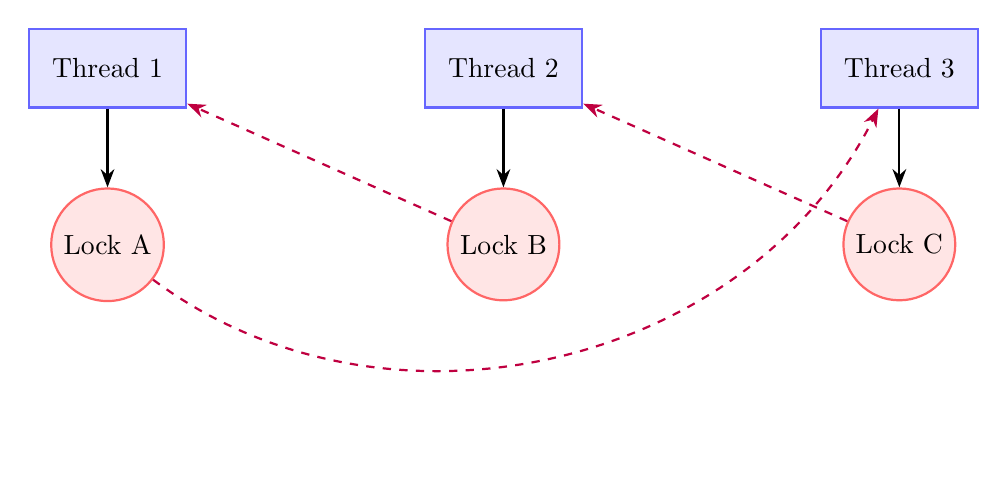
\begin{tikzpicture}[
      thread/.style={rectangle, draw=blue!60, fill=blue!10, thick, minimum width=2cm, minimum height=1cm},
      lock/.style={circle, draw=red!60, fill=red!10, thick, minimum size=1cm},
      arrow/.style={->, thick, >=Stealth}
      ]

      % Nodes
      \node[thread] (T1) {Thread 1};
      \node[lock, below=of T1] (A) {Lock A};

      \node[thread, right=3cm of T1] (T2) {Thread 2};
      \node[lock, below=of T2] (B) {Lock B};

      \node[thread, right=3cm of T2] (T3) {Thread 3};
      \node[lock, below=of T3] (C) {Lock C};

      % Arrows
      \draw[arrow] (T1) -- (A);
      \draw[arrow] (T2) -- (B);
      \draw[arrow,purple,dashed] (B) -- (T1);
      \draw[arrow] (T3) -- (C);
      \draw[arrow,purple,dashed] (C) -- (T2);
      \draw[arrow,purple,dashed] (A) to[bend right=50] (T3);

    \end{tikzpicture}
  \end{center}

  \begin{block}<2->{\faPuzzlePiece \quad What is wrong?}
    A more complex cyclic dependency!
  \end{block}

\end{frame}

\begin{frame}[fragile]
  \frametitle{\faSkull \quad Deadlock example (3)}

\begin{lstlisting}[basicstyle=\fontsize{8}{9}\selectfont\ttfamily, language = Java ,
frame = trBL , firstnumber = last , escapeinside={(*@}{@*)},numbers=none]
class Safe {
    synchronized void unlock() {
        Database.logAccess(this);  // External method call while holding lock!
    }
}
class Database {
    static synchronized void logAccess(Safe s) {
        System.out.println("Accessing safe %n", s.id);
    }
}
\end{lstlisting}



  \begin{block}<3->{\faPuzzlePiece \quad What's going on?}
    \uncover<4->{Imagine a thread calling \texttt{unlock()}, while another that already holds
    the (shared) \texttt{Database} lock, tries to use some synchronized class on
    the same instance of \texttt{Safe}.}
  \end{block}

  \begin{block}<4->{\faLightbulb \quad Key takeaway}
    Calling external synchronized methods while holding a lock is dangerous.
  \end{block}

      \uncover<2->{
    \begin{tikzpicture}[overlay, remember picture]
      \node[xshift=10.4cm,yshift=7cm,starburst,starburst points=20,
      align=center,fill=yellow, opacity=1,draw=red, line width=2pt]
      {\textbf{Closed call!}};
    \end{tikzpicture}}
\end{frame}

\begin{frame}[fragile]
  \frametitle{\faSkull \quad Deadlock example (4)}

\begin{lstlisting}[basicstyle=\fontsize{8}{9}\selectfont\ttfamily, language = Java ,
frame = trBL , firstnumber = last , escapeinside={(*@}{@*)},numbers=none]
  public void transferMoney(Account fromAcc, Account toAcc, DollarAmount amount) {
    synchronized (fromAcc) {
      synchronized (toAcc) {
        if (fromAcc.hasSufficientBalance(amount) {
          fromAcc.debit(amount);
          toAcc.credit(amount);
        }
      }
    }
  }
\end{lstlisting}

  \begin{block}<2->{\faPuzzlePiece \quad What's going on?}
    \uncover<3->{The order of lock acquisition depends on the \emph{caller}.}
    \uncover<4->{If a thread calls \texttt{transferMoney}(acc1, acc2, amount1)
      and another \texttt{transferMoney}(acc2, acc1, amount2), you may run into
    a deadlock!}
  \end{block}
\end{frame}

\begin{frame}[fragile]
  \frametitle{\faSkull \quad Deadlock example (4), rectified}

\begin{lstlisting}[basicstyle=\fontsize{8}{9}\selectfont\ttfamily, language = Java ,
frame = trBL , firstnumber = last , escapeinside={(*@}{@*)},numbers=none]
 public void transferMoney(Account fromAcc, Account toAcc, DollarAmount amount) {
    Account firstLock, secondLock;
    if (fromAcc.accountNumber() == toAcc.accountNumber())
      throw new Exception("Cannot transfer from account to itself");
    else if (fromAcc.accountNumber() < toAcc.accountNumber()) {
      firstLock = fromAcc; secondLock = toAcc;
    }
    else {
      firstLock = toAcc; secondLock = fromAcc;
    }
    synchronized (firstLock) {
      synchronized (secondLock) {
        if (fromAcc.hasSufficientBalance(amount) {
          fromAcc.debit(amount);
          toAcc.credit(amount);
        }
      }
    }
  }
\end{lstlisting}
\end{frame}

\begin{frame}[fragile]
  \frametitle{\faBriefcaseMedical \quad Avoiding Deadlocks}

  \begin{block}{\faExclamationTriangle \quad Remember}
    Deadlocks, i.e. potential cyclic dependencies in locks, can be buried very
    deeply in the code. It is thus important to practice extra care when you
    work with multiple locks.
  \end{block}

  Here are some tips to avoid deadlocks:

  \begin{itemize}
  \item[\faBook]<2-> Enforce a global order on lock acquisition!
  \item[\faBook]<3-> Use \texttt{tryLock} that allow a thread to stop waiting
    after user-supplied timeout. This way you can detect potential deadlocks
    based on the failure of \texttt{tryLock}.
  \item[\faBook]<4-> Use \textbf{open calls} instead of the risky closed calls.
  \end{itemize}

\end{frame}

\begin{frame}[fragile]
  \frametitle{Starvation}

  \begin{block}<1->{\faSearch \quad What is starvation?}
    The situation where a thread/task is constantly denied access to resources to
    function (e.g. a lock, CPU time) because of other threads.
  \end{block}
  \vspace{0.5cm}
  \begin{block}<2->{\faSearch \quad When does it occur?}
    By inappropriate use of thread (OS-level) or \textbf{task} priorities.
  \end{block}
  \vspace{0.5cm}
  \begin{block}<3->{\faSearch \quad Real-world example}
    Waiting forever in the emergency room in a hospital because more serious
    cases keep coming up. \uncover<4->{We've all been there.}
  \end{block}
\end{frame}

\begin{frame}[fragile]
  \frametitle{Starvation example}

  \centering \huge
  Live demo

\end{frame}

\begin{frame}[fragile]
  \frametitle{Avoiding Starvation}

  \begin{block}{\faExclamationTriangle \quad Remember}
    Starvations are all about improper handling of task/thread priority.
  \end{block}

  Here are some tips to avoid starvation:

  \begin{itemize}
  \item[\faBook]<2-> Resist the temptation to use OS-level priorities.
  \item[\faBook]<3-> Design and implement your task priority carefully. Be
    careful of \textbf{retry-storms}.
  \item[\faBook]<4-> If all tasks have equal priority, make sure your code does
    not introduce implicit prioritization.
  \end{itemize}

\end{frame}



\begin{frame}[fragile]
  \frametitle{Livelock}

  \begin{block}<1->{\faSearch \quad What is a livelock?}
    A livelock occurs when two or more threads repeat the same interaction in
    response to changes in the state of other processes, but no progress is
    made. \uncover<2->{According to Goetz, a livelock can also occur to a
      single-thread in a kind of \emph{poison-message} scenario, where a
      thread \emph{independently} retries an operation.}
  \end{block}
  \vspace{0.5cm}
  \begin{block}<3->{\faSearch \quad Real-world example}
    Two friends keep calling each other because the line is busy.
    \uncover<4->{We've all been there.}
  \end{block}

\end{frame}

\begin{frame}[fragile]
  \frametitle{Livelock example}

  \centering \huge
  Live demo

\end{frame}

\begin{frame}[fragile]
  \frametitle{Avoiding livelocks}

  \begin{block}{\faExclamationTriangle \quad Remember}
    Livelocks often occur because of a very eager retry strategy.
  \end{block}

  Hence, to avoid livelocks, one has to avoid retry storms by...

  \begin{itemize}
  \item[\faBook]<2-> Limiting the number of retries.
  \item[\faBook]<3-> Backing off after no progress has been detected.
  \end{itemize}

\end{frame}

\begin{frame}[fragile]
  \frametitle{Liveness recap}

  \begin{table}[h]
    \centering
    \begin{tabularx}{\textwidth}{|l|c|c|c|X|}
      \hline
      \textbf{Hazard} & \textbf{Symptom} & \textbf{Blocking?} & \textbf{Active?}
      & \textbf{Example} \\
      \hline
      Deadlock & No progress & Yes & No & Two threads jointly waiting for locks
                                          that are held by the other.
      \\
      \hline
      Starvation & $\leq 1$ Threads stuck & No & Others
      & Greedy thread hogs lock or other resource. \\
      \hline
      Livelock & Constant retrying & No & Yes & Two threads yielding to each other.\\
      \hline
    \end{tabularx}
    \caption{Comparison of liveness hazards.}
  \end{table}
\end{frame}

\section{Performance and Scalability}

\begin{frame}[fragile]
  \frametitle{Performance and scalability}

  \begin{block}<1->{\faFlagCheckered \quad What is a performance?}
    How fast is a system. Measures include \textbf{throughput} (tasks completed
    per unit time) and \textbf{latency} (time to complete a task). \textbf{How fast?}
  \end{block}

  \vspace{0.4cm}

  \begin{block}<2->{\faMountain \quad What is scalability?}
    Measures the ability to improve throughput or capacity when
    additional computing resources (such as additional CPUs, memory etc.) are
    added. \textbf{How much?}
  \end{block}

  \vspace{0.4cm}

  \begin{block}<3->{\faLightbulb \quad Performance vs scalability}
    Performance and scalability are separate measurements, often at odds. For
    instance, many tricks that improve raw performance (e.g. caching) hurt
    scalability.
  \end{block}
\end{frame}

\begin{frame}[fragile]
  \frametitle{A common ground}

  In concurrency, I find that performance and scalability both generally boil down to one
  common, critical parameter.

  \vspace{0.6cm}

  \begin{block}<2->{\faLightbulb \quad Utilization}
    Efficient, scalable concurrent programming relies on maximizing the amount
    of utilization of system resources (e.g. CPU power first and foremost).
  \end{block}
\end{frame}

\begin{frame}[fragile]
  \frametitle{Performance and scalability vs parallelism}
\begin{itemize}
\item[\faBook]<1-> At the beginning, I made a big fuss over concurrent
  programming  not being the same as parallel programming.
\item[\faBook]<2-> This is true, especially conceptually.
\item[\faBook]<3-> However, being able to make efficient use of the
  computational resources in a concurrent scenario hinges on
  \emph{parallelism}.
  \begin{itemize}
  \item[\faBook]<3-> Identifying the sources of serialization and the
    independent, parallelizable parts.
  \item[\faBook]<3-> Using all available CPU threads.
  \end{itemize}
\item[\faBook]<4-> Hence, parallelism \emph{encourages} concurrency.
\end{itemize}

\end{frame}

\begin{frame}[fragile]
  \frametitle{Recall Week 14}

  \begin{block}<1->{\faLightbulb \quad Key takeaway}
    The larger the serialized part is, the less one stands to gain from parallelism.
  \end{block}

  \vspace{0.6cm}

  \begin{block}<2->{\faLightbulb \quad Amdahl's law}
    \[
      \mathrm{Speedup} \leq \frac{1}{F + \frac{1-F}{N}}
    \]
    In the above, $N$ is the number of threads and $F$ the \emph{fraction} of
    the \emph{serialized} code.
  \end{block}
\end{frame}

\begin{frame}[fragile]
  \frametitle{Amdahl's law}

  \begin{center}
    \includegraphics[width=10cm,keepaspectratio]{../media/Amdahls.png}
  \end{center}

\end{frame}

\begin{frame}[fragile]
  \frametitle{Tips and tricks}

  \begin{itemize}
  \item[\faBook]<1-> Break locks into smaller ones.
  \item[\faBook]<1-> Reduce critical sections.
  \item[\faBook]<1-> Use non-blocking data structures.
  \item[\faBook]<1-> Use non-blocking data structures.
  \item[\faBook]<1-> Use atomic variables (e.g., \texttt{AtomicInteger}).
  \item[\faBook]<1-> Use \texttt{ReadWriteLock} if reads dominate.
  \item[\faBook]<1-> Use lock-free and wait-free algorithms.
  \item[\faBook]<1-> Prefer short-lived, non-blocking tasks.
  \item[\faBook]<1-> Avoid "synchronized(this)" on large classes.
  \item[\faBook]<1-> Design systems to degrade gracefully under load.
  \end{itemize}

\end{frame}

\begin{frame}[fragile]
  \frametitle{Recap}

  \begin{itemize}
  \item[\faBook]<1-> Scalability = Concurrency done well.
  \item[\faBook]<1-> Minimize blocking, contention, and switching.
  \item[\faBook]<1-> Think about critical paths and Amdahl’s Law.
  \item[\faBook]<1-> Good concurrency = smarter designs, not just "more threads".
  \end{itemize}

\end{frame}

\section{(Parallel) Streams}

\begin{frame}[fragile]
  \frametitle{More general than you think}
  \begin{itemize}
  \item[\faBook]<1-> At a glance, Streams feel very specific.
  \item[\faBook]<2-> However, almost every interaction of the computer with the
    outer world boils down to \emph{files} and \emph{streams}.
  \item[\faBook]<3-> In fact, the file is one of the two core
    concepts and programming structure of Operating Systems, the other being the process.
  \end{itemize}

  \vspace{0.6cm}

  \begin{block}<4->{\faLightbulb \quad How about Parallel Streams?}
    \uncover<5->{Also general! They manifest the \textbf{MapReduce} paradigm for
    Java!}
  \end{block}
\end{frame}

\begin{frame}[fragile]
  \frametitle{MapReduce?}

  \begin{block}<1->{\faLightbulb \quad What is the MapReduce paradigm?}
    The MapReduce paradigm applies to the (very) broad class of problems whose
    input data is a large collection and their solutions have this pattern:
    \begin{enumerate}
    \item A uniform operation (or a sequence) is applied to every element
      of the collection (\textbf{Map} in \textbf{Map}Reduce).
    \item The results are then aggregated together via a method of
      \emph{reduction} (\textbf{Reduce} in Map\textbf{Reduce}.)
    \end{enumerate}
  \end{block}

\end{frame}

\section{Some info on the Exam}

\begin{frame}[fragile]
  \frametitle{Exam info}

  \begin{itemize}
  \item[\faBook]<1-> One large Java file.
  \item[\faBook]<1-> Visit
    \href{https://github.com/fmontesi/cp-2024/tree/main/exam}{https://github.com/fmontesi/cp-2024/tree/main/exam}
    for last year's exam.
  \item[\faBook]<1-> This year's exam will follow a similar recipe.
  \item[\faBook]<1-> What matters is code quality and demonstrating good
    command of what we have covered.
  \item[\faBook]<1-> Correctness is more important than speed (you need to use
    concurrent methods, of course).
  \item[\faBook]<1-> We will discuss more next week.
  \end{itemize}

\end{frame}

\begin{frame}[fragile]
  \frametitle{Examples  used in the lecture}

  \begin{itemize}
  \item[\faCode]<1-> Week18/Starvation/TaskQueueDemo.java : example of
    starvation.
  \item[\faCode]<1-> Week18/Livelock/PhilosopherDemo.java : demonstrating a
    livelock using ``polite'' philosophers.
  \item[\faCode]<1-> Week18/Streams/* : examples with parallel Streams.
  \end{itemize}

\end{frame}

\begin{frame}{}
  \centering \huge
  Thank you!
\end{frame}

\end{document}

%%% Local Variables:
%%% mode: latex
%%% TeX-engine: xetex
%%% TeX-master: t
%%% End:
